\documentclass[11pt,a4paper]{article}

\usepackage[utf8]{inputenc}
\usepackage[T1]{fontenc}
\usepackage[brazilian]{babel}
\usepackage{geometry}
\usepackage{graphicx}
\usepackage{booktabs}
\usepackage{amsmath}
\usepackage{float}
\usepackage{hyperref}

\geometry{margin=2.4cm}
\hypersetup{hidelinks}
\setlength{\parskip}{0.45em}
\setlength{\parindent}{0pt}

\title{DBO na entrada com 10 DBO medidas\\[0.3em]
\large Rede recorrente e a fila de laboratório}
\author{SoftSensor}
\date{16 de outubro de 2026}

\begin{document}
\maketitle

\section{Objetivo}

Estimar a DBO na entrada da estação, \texttt{DBO-E}. A diferença em relação à RNN anterior é a fila. Cada exemplo guarda 10 valores reais de DBO, os dez dias anteriores disponíveis. A DBO do dia estimado não entra nessa fila.

A DQO (\texttt{DQO-E}) e o SST (\texttt{SS-E}) do dia estimado continuam na saída, junto com o estado final da rede. São as medidas desse dia. As leituras anteriores de DQO e de SST não são guardadas.

\section{Dados e janela}

O conjunto é o Water Treatment Plant, de Manel Poch (UCI, 1993). São 527 dias. Ficam 498 dias em que \texttt{DBO-E}, \texttt{DQO-E} e \texttt{SS-E} existem juntos; 29 dias saem por valor ausente. Não há interpolação. As unidades não estão documentadas na UCI.

A fila segue a próxima leitura disponível, não o dia de calendário seguinte. O intervalo mediano entre leituras é 1 dia. Em 116 pares o intervalo passa de um dia, e o maior é de 32 dias. As 10 DBO anteriores cobrem, na mediana, 11 dias de calendário, e no máximo 43.

A série vai de 1 de janeiro de 1990 a 29 de outubro de 1991. A DBO média dos alvos de treino é 194,93, com desvio 66,28. Nos 100 dias de teste, a partir de 29 de maio de 1991, a média cai para 163,77 e o desvio cai para 36,63.

\section{Protocolo}

Os 398 dias mais antigos treinam. Os 100 mais recentes testam. A divisão é cronológica e é a mesma dos 100 dias finais da RNN de DQO e SST. Surgem 388 janelas de treino, porque as dez primeiras leituras só entram como histórico, e 100 janelas de teste. A primeira janela de teste usa as últimas DBO do treino como histórico. O alvo dela já é um dia de teste.

A validação cruzada fica restrita ao treino e também é temporal (\texttt{TimeSeriesSplit}, 5 partições). O critério é o MAE. Dentro de cada partição, a padronização usa só as janelas de treino daquela partição. A DBO da fila e a DBO alvo compartilham o mesmo scaler.

A rede é uma RNN de Elman: uma camada recorrente com tangente hiperbólica lê as 10 DBO em ordem, e uma saída linear junta o estado final à DQO e ao SST do dia. O treino é Adam, com retropropagação no tempo e corte de gradiente. A grade cobre estados de 8, 16 e 32 unidades e taxas de aprendizado \(10^{-3}\) e \(10^{-2}\). O ajuste final repete, em todas as janelas de treino, o número mediano de épocas em que a configuração vencedora parou na validação.

Cinco referências usam o mesmo corte: a média da DBO de treino, a DBO medida imediatamente anterior, a regressão linear só com a DQO e o SST do dia, a regressão linear com as 10 DBO anteriores e a regressão linear com essas 10 DBO mais a DQO e o SST do dia.

\section{Resultados}

A validação escolhe estado de 8 unidades e taxa \(10^{-2}\). O MAE nas partições é 40,20, com desvio 2,77. A parada ocorre em 8 épocas. A rede tem 91 parâmetros. As seis configurações ficam entre 40,20 e 46,84 de MAE: aumentar o estado não reduz o erro.

\begin{table}[H]
\centering
\caption{Erro nos 100 dias finais, de 29 de maio a 29 de outubro de 1991. ``DBO anterior'' repete a última DBO medida. ``DQO e SST do dia'' é a reta só com as duas medidas do dia estimado.}
\begin{tabular}{lrrr}
\toprule
Modelo & MAE & RMSE & \(R^{2}\) \\
\midrule
Média do treino & 40,83 & 48,09 & $-$0,72 \\
DBO anterior & 35,85 & 44,48 & $-$0,47 \\
DQO e SST do dia & 33,13 & 40,76 & $-$0,24 \\
10 DBO anteriores & 30,45 & 37,12 & $-$0,03 \\
10 DBO + DQO e SST & 26,86 & 34,41 & 0,12 \\
RNN & 25,69 & 33,52 & 0,16 \\
\bottomrule
\end{tabular}
\end{table}

A reta com as 10 DBO anteriores, a DQO e o SST do dia é
\begin{equation}
\widehat{\mathrm{DBO}} = 6{,}87 + \sum_{k=1}^{10} \beta_k \,\mathrm{DBO}_{t-k} + 0{,}2363\,\mathrm{DQO} - 0{,}0070\,\mathrm{SST}.
\end{equation}
O coeficiente da DBO de ontem é 0,195, o de dois dias atrás é 0,113 e o de três dias é 0,068. Os lags mais antigos oscilam em torno de zero. A soma dos dez coeficientes de DBO é 0,476. A DQO do dia, 0,236, é o maior coeficiente isolado. O SST fica em $-$0,007.

No teste, a previsão da RNN vai de 105,72 a 250,70, e a DBO observada vai de 84 a 277. O resíduo médio (observado menos previsto) é $-$8,80. Nos dez primeiros dias de teste é $-$6,78; nos noventa seguintes, $-$9,02. A mediana do erro absoluto é 19,78 e o percentil 90 é 55,68. Em 65 dos 100 dias o erro absoluto fica até 30; em 86 dias, até 50.

\begin{figure}[H]
\centering
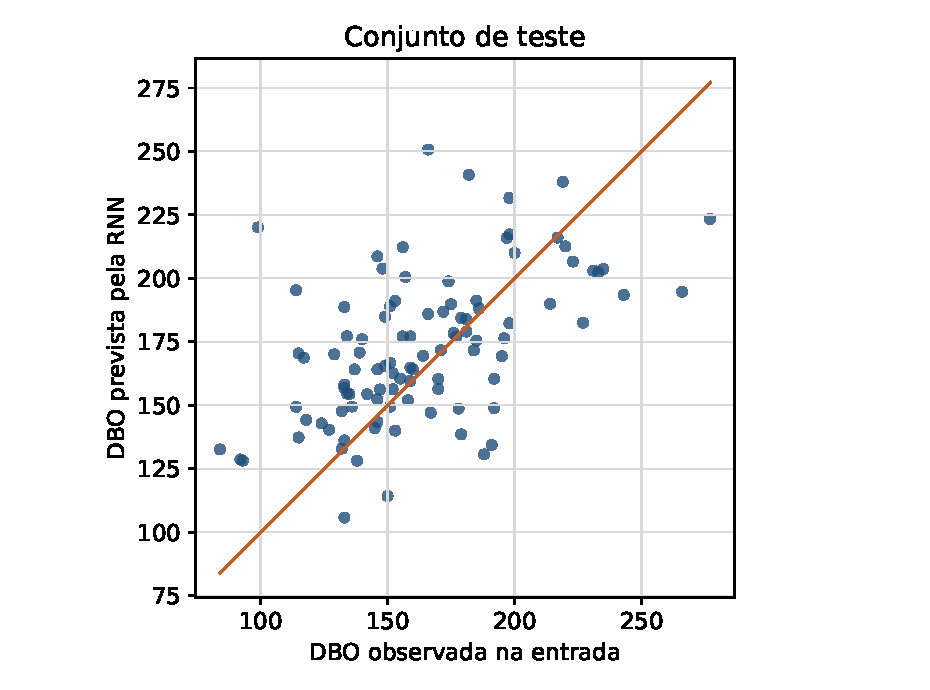
\includegraphics[width=0.72\textwidth]{figuras/rnn_dbo_anteriores_observado.pdf}
\caption{Teste da RNN. A reta marca a previsão igual à observação. A nuvem acompanha a reta e ainda se espalha: vários dias de DBO baixa são previstos acima dela.}
\label{fig:previsto}
\end{figure}

\begin{figure}[H]
\centering
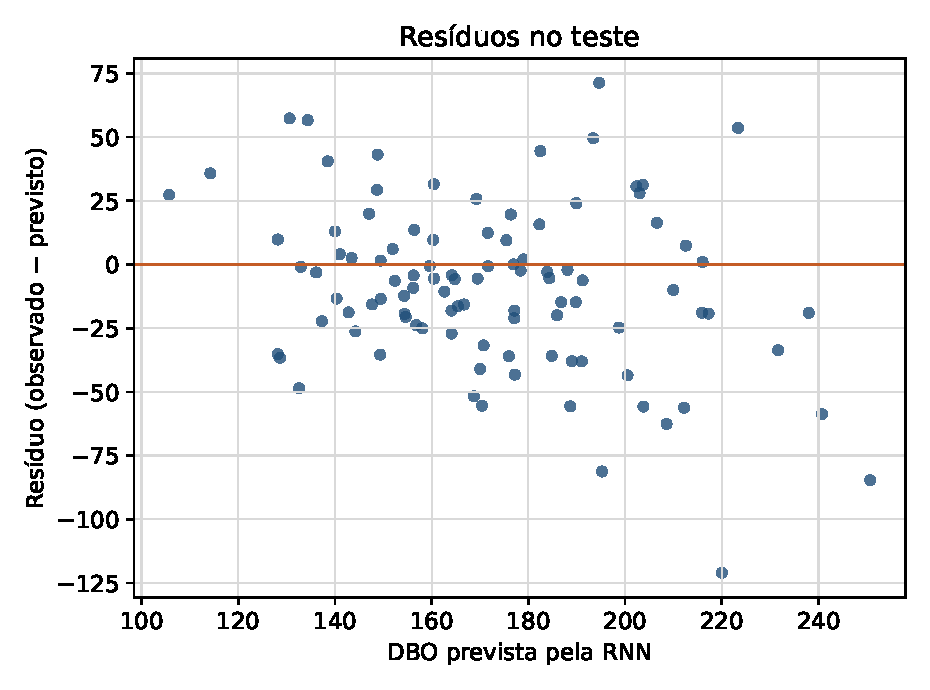
\includegraphics[width=0.72\textwidth]{figuras/rnn_dbo_anteriores_residuos.pdf}
\caption{Resíduos no teste. O centro fica um pouco abaixo de zero. Os maiores desvios passam de 50, e um dia passa de 100.}
\label{fig:residuos}
\end{figure}

\begin{figure}[H]
\centering
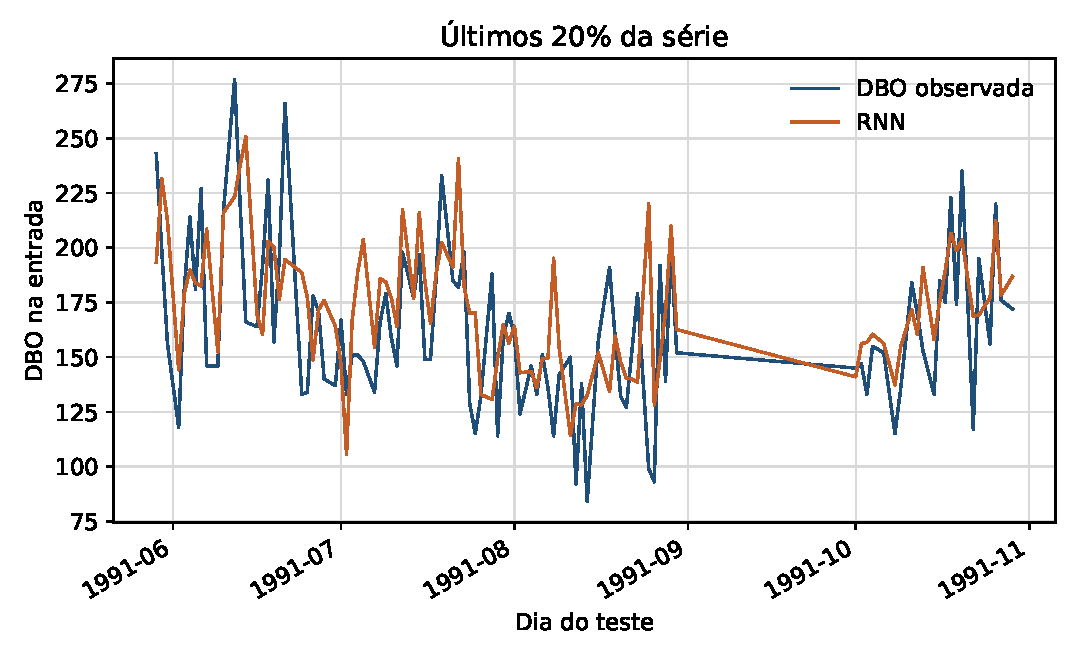
\includegraphics[width=0.92\textwidth]{figuras/rnn_dbo_anteriores_serie.pdf}
\caption{Os 100 dias de teste. A RNN segue o sobe e desce da DBO medida e perde os picos mais agudos. Um trecho longo e quase reto é um intervalo sem medida, não uma DBO constante.}
\label{fig:serie}
\end{figure}

\section{Leitura}

Esta RNN vê uma informação que a RNN de DQO e SST não via: a DBO de laboratório dos dias anteriores. Nos mesmos 100 dias, aquela rede tinha MAE 32,00, RMSE 40,68 e \(R^{2}\) $-$0,23, e ficava em média 22 unidades acima da medida. Aqui o MAE cai para 25,69, o RMSE para 33,52 e o \(R^{2}\) passa a 0,16. O viés cai para cerca de 9 unidades. A comparação não diz que a recorrência ficou mais capaz. Diz que a DBO já medida muda o problema.

A queda não vem de repetir a última DBO. Essa persistência tem MAE 35,85, pior do que a reta da DQO e do SST do dia (33,13). O dia a dia da entrada salta mais do que a DQO consegue acompanhar, e um único valor anterior não segura o nível.

O que os coeficientes sustentam é uma mistura. As 10 DBO, sozinhas, chegam a MAE 30,45. Juntas com a DQO e o SST do dia, chegam a 26,86. A RNN fica em 25,69. A margem de 1,17 sobre a reta cabe dentro do desvio de 2,77 da validação. O estado de 8 unidades vence os de 16 e 32. A rede reproduz, com pouca folga, a combinação linear.

A soma 0,476 dos coeficientes de DBO explica o viés que sobra. Se o patamar cai e a fila só carrega cerca de metade dessa queda, a outra metade continua na previsão. A DQO do dia, com coeficiente 0,236, puxa para a relação antiga, a mesma reta de intercepto 73 que já aparecia sem histórico de DBO. O viés dos dez primeiros dias de teste ($-$6,78) e o dos noventa seguintes ($-$9,02) são parecidos: não é a fila ainda cheia do patamar de treino. É a fila, já dentro do período baixo, que só acompanha parte do nível.

O SST segue sem papel. O coeficiente é $-$0,007, na mesma ordem do que se via na RNN anterior.

O \(R^{2}\) de 0,16 é o primeiro positivo neste corte cronológico. A previsão fica melhor do que usar a média dos próprios dias de teste. Ainda assim, a maior parte da variação desses cem dias continua fora do modelo. A mediana do erro é 20, o erro médio é 26, cerca de 16\% da DBO média do teste (164), e em um de cada dez dias o erro passa de 56. A faixa prevista, de 106 a 251, não cobre a observada, de 84 a 277. A Figura~\ref{fig:serie} mostra o acompanhamento do traço e a perda dos picos. A Figura~\ref{fig:previsto} mostra a nuvem ainda larga.

Há um limite de uso. Para estimar o dia de hoje, o modelo precisa das 10 últimas DBO de laboratório. Se essas análises já chegaram, a fila ajuda. Se o soft sensor existe justamente para não esperar a DBO, a referência continua sendo a reta da DQO e do SST, com MAE 33,13 neste corte.

\section{Conclusão}

Com 10 DBO medidas anteriores, mais a DQO e o SST do dia, a RNN de 8 unidades chega a MAE 25,69, RMSE 33,52 e \(R^{2}\) 0,16 nos 100 dias finais. É o menor erro entre os modelos deste corte, e fica à frente da RNN que só via DQO e SST (MAE 32,00 e \(R^{2}\) $-$0,23). A regressão linear com a mesma fila e as mesmas duas medidas do dia fica ao lado, com MAE 26,86 e RMSE 34,41.

Os resultados chegam mais perto da DBO alvo e ainda estão distantes dela. O erro típico fica em 20, o erro médio em 26, e um em cada dez dias erra 56 ou mais. A previsão continua cerca de 9 unidades acima da medida, porque a fila só carrega metade da mudança de nível e a DQO segura a escala antiga. O centro da série é acompanhado. O pico, o vale e o patamar completo não são.

O notebook é \texttt{rnn\_dbo\_anteriores.ipynb}, na pasta \texttt{modelo}. A RNN só com DQO e SST está em \texttt{rnn\_dbo\_entrada.pdf}, na pasta \texttt{docs}.
\end{document}
